

\tikzset{every picture/.style={line width=0.75pt}} %set default line width to 0.75pt        

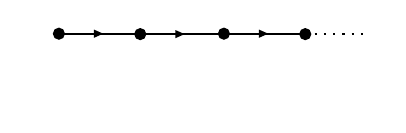
\begin{tikzpicture}[x=0.75pt,y=0.75pt,yscale=-1,xscale=1]
%uncomment if require: \path (0,300); %set diagram left start at 0, and has height of 300

%Straight Lines [id:da6276790682079358] 
\draw    (100.6,110) -- (140.85,110) ;
%Straight Lines [id:da6334935852876922] 
\draw    (180.1,110) -- (220.35,110) ;
%Straight Lines [id:da8191358904406301] 
\draw    (139.8,110.2) -- (180.05,110.2) ;
%Straight Lines [id:da9015443131541547] 
\draw  [dash pattern={on 0.84pt off 2.51pt}]  (219.3,110.2) -- (250.15,110.2) ;


%Flowchart: Connector [id:dp10712755168097865] 
\draw  [fill={rgb, 255:red, 0; green, 0; blue, 0 }  ,fill opacity=1 ] (103,110) .. controls (103,111.33) and (101.93,112.4) .. (100.6,112.4) .. controls (99.27,112.4) and (98.2,111.33) .. (98.2,110) .. controls (98.2,108.67) and (99.27,107.6) .. (100.6,107.6) .. controls (101.93,107.6) and (103,108.67) .. (103,110) -- cycle ;
%Flowchart: Connector [id:dp9628511983929124] 
\draw  [fill={rgb, 255:red, 0; green, 0; blue, 0 }  ,fill opacity=1 ] (142.2,110.2) .. controls (142.2,111.53) and (141.13,112.6) .. (139.8,112.6) .. controls (138.47,112.6) and (137.4,111.53) .. (137.4,110.2) .. controls (137.4,108.87) and (138.47,107.8) .. (139.8,107.8) .. controls (141.13,107.8) and (142.2,108.87) .. (142.2,110.2) -- cycle ;
%Flowchart: Connector [id:dp022374442404981654] 
\draw  [fill={rgb, 255:red, 0; green, 0; blue, 0 }  ,fill opacity=1 ] (182.5,110) .. controls (182.5,111.33) and (181.43,112.4) .. (180.1,112.4) .. controls (178.77,112.4) and (177.7,111.33) .. (177.7,110) .. controls (177.7,108.67) and (178.77,107.6) .. (180.1,107.6) .. controls (181.43,107.6) and (182.5,108.67) .. (182.5,110) -- cycle ;
%Flowchart: Connector [id:dp8113410302855639] 
\draw  [fill={rgb, 255:red, 0; green, 0; blue, 0 }  ,fill opacity=1 ] (221.7,110.2) .. controls (221.7,111.53) and (220.63,112.6) .. (219.3,112.6) .. controls (217.97,112.6) and (216.9,111.53) .. (216.9,110.2) .. controls (216.9,108.87) and (217.97,107.8) .. (219.3,107.8) .. controls (220.63,107.8) and (221.7,108.87) .. (221.7,110.2) -- cycle ;

%Shape: Triangle [id:dp18185199166706778] 
\draw  [color={rgb, 255:red, 0; green, 0; blue, 0 }  ,fill opacity=1 ][fill={rgb, 255:red, 0; green, 0; blue, 0 }  ,fill opacity=1 ] (120.72,110) -- (118,111.21) -- (118,108.79) -- cycle ;
%Shape: Triangle [id:dp11767706980455106] 
\draw  [color={rgb, 255:red, 0; green, 0; blue, 0 }  ,draw opacity=1 ][fill={rgb, 255:red, 0; green, 0; blue, 0 }  ,fill opacity=1 ] (159.92,110.2) -- (157.2,111.41) -- (157.2,108.99) -- cycle ;
%Shape: Triangle [id:dp5972516863295354] 
\draw  [color={rgb, 255:red, 0; green, 0; blue, 0 }  ,fill opacity=1 ][fill={rgb, 255:red, 0; green, 0; blue, 0 }  ,fill opacity=1 ] (200.22,110) -- (197.5,111.21) -- (197.5,108.79) -- cycle ;

\draw (250,140) node   {};
\draw (90,140) node   {};


\end{tikzpicture}

